%\info{Andrew, Simone}

Having defined the observables and grooming procedures of interest, in this section we provide a general discussion of the potential advantages of the use of groomed jet observables for measurements of $\alpha_s$. The grooming procedure significantly simplifies a number of theoretical and experimental issues related to precision calculations and measurements in a $pp$ environment. In particular, grooming provides
\begin{itemize}
\item Mitigation of NP effects
\item Perturbative simplicity
\item Improved detector resolution, due in large part to a reduced pileup sensitivity
\end{itemize}
Each of these will be discussed in more detail in the following
sections.  Combined, we believe that they provide a strong case for
the interest in the measurement of the groomed jet observables, and the possibility of performing a
precision extraction of $\alpha_s$ using jet substructure at the LHC.




%%%%%%%%%%%%%%%%%%%%%%%%%%%%%%%%%%%%%
\subsection{Mitigating Nonperturbative Effects ($e^+e^-$ and $pp$)}
%%%%%%%%%%%%%%%%%%%%%%%%%%%%%%%%%%%%%

One of the primary complications of $\alpha_s$ extractions using event
shapes is the challenge of NP corrections, which cannot
currently be calculated from first principles. Since event shape
observables probe singular regions of the phase space, they are
necessarily sensitive to non-perturbative corrections.  For $e^+e^-$
dijet event shapes, such as thrust, these non-perturbative corrections
can be given operator definitions in the dijet limit. Although these
operators cannot be calculated, they can be modeled using \textit{shape functions}\footnote{There are other approaches to analytically describe and fit NP effects that have similar features to shape functions.  Another example is the dispersive model~\cite{Dokshitzer:1995qm,Dokshitzer:1995zt} which has also been used to make extractions of $\alpha_s$ using $e^+e^-$ event shapes~\cite{Gehrmann:2012sc}.}
\cite{Korchemsky:1999kt,Korchemsky:2000kp,Hoang:2007vb,Ligeti:2008ac}. These
shape functions can be systematically expanded in moments, and for
moderately large values of the observable, only the first moment,
$\Omega_1$ is required. This moment can be shown to be universal for a
wide range of observables \cite{Lee:2006fn,Lee:2007jr}, and can
therefore be extracted from data along with $\alpha_s$
\cite{Abbate:2010xh,Abbate:2012jh,Hoang:2015hka}. However, this moment
is highly correlated with $\alpha_s$ as shown in \Fig{fig:correlation_firstmoment}. Therefore, observables with
different, and preferably suppressed non-perturbative effects could
provide valuable complementary information for $\alpha_s$ extractions.
%

  
  % introducing uncertainties into the extraction. Furthermore, there is disagreement over whether the use of a single shape function moment is applicable in the region where $\alpha_s$ fits are performed~\cite{}

\begin{figure}
\begin{center}
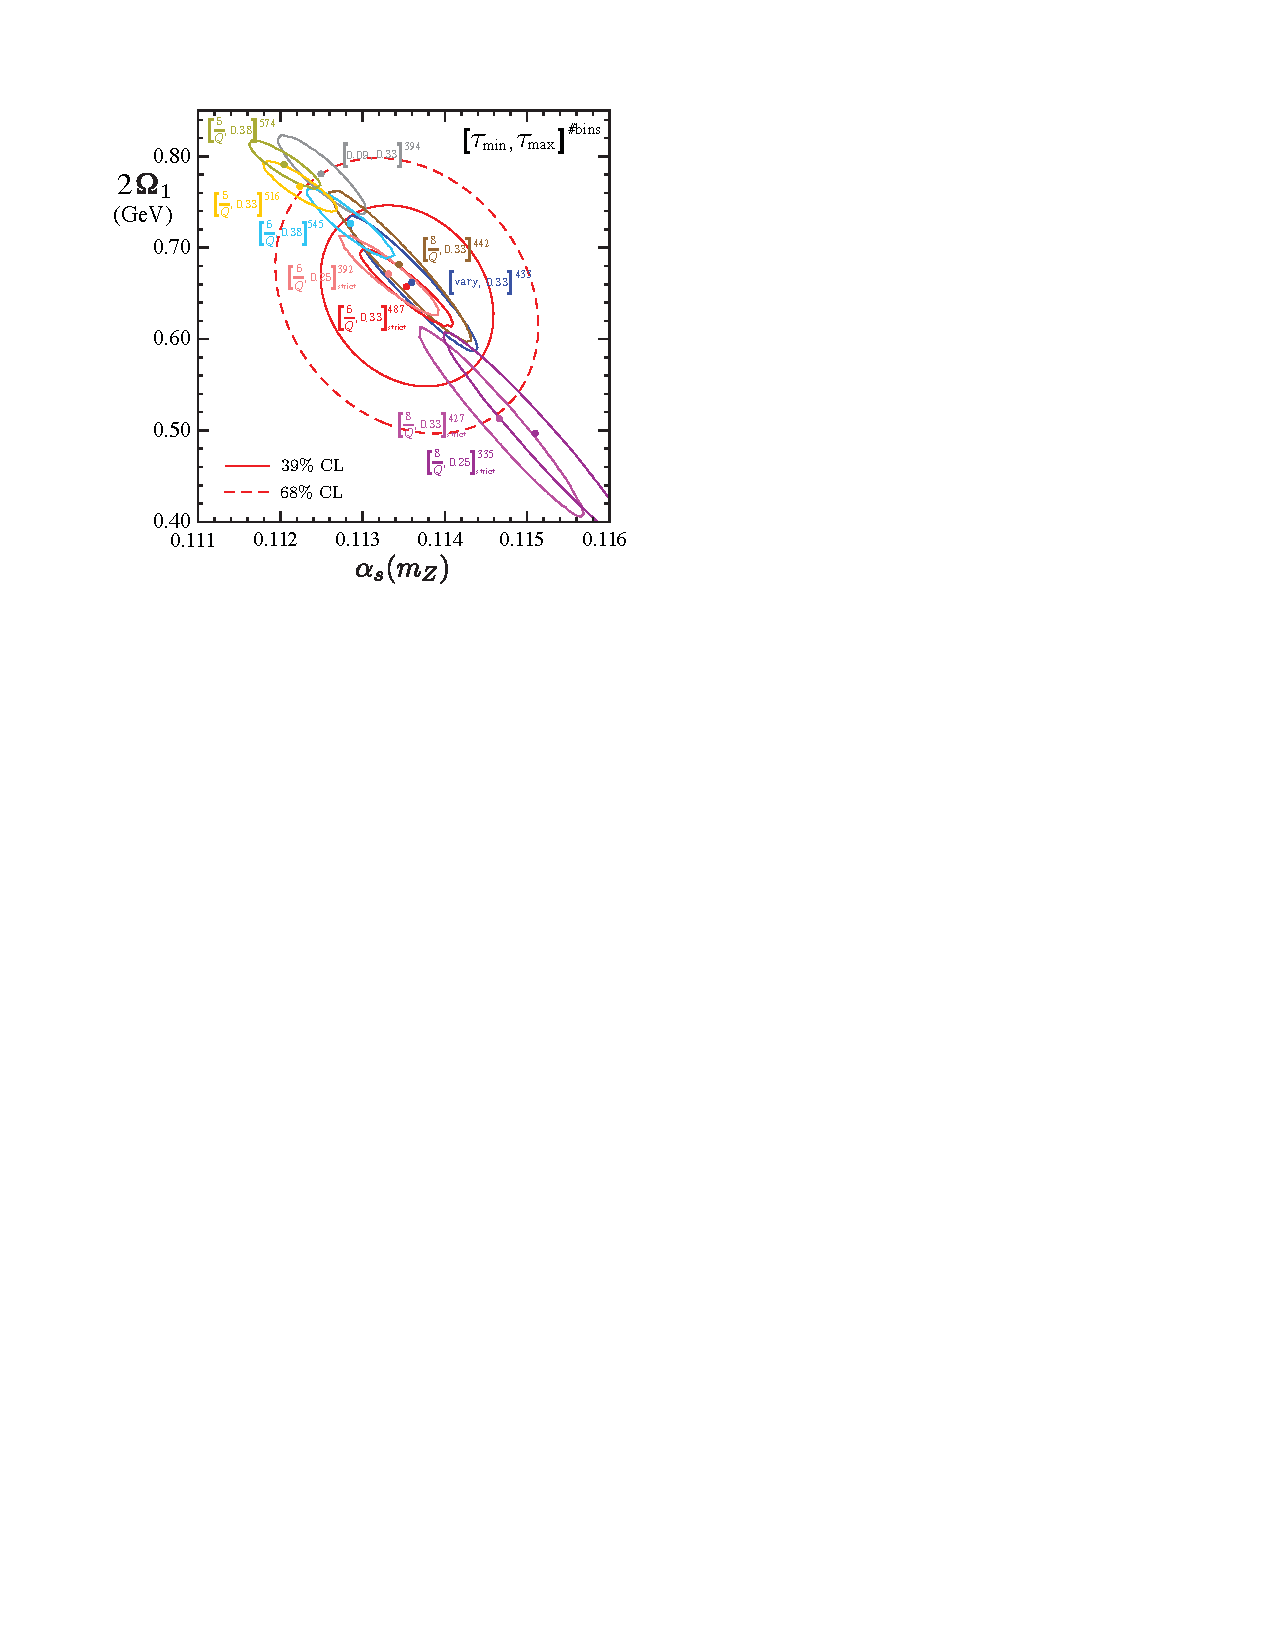
\includegraphics[width = 0.6\columnwidth]{figures/correlation_firstmoment.pdf}
\end{center}
\caption{An illustration of the correlations between the first non-perturbative moment $\Omega_1$ and $\alpha_s$ for the thrust observables. Non-perturbative effects for groomed observables have a significantly different structure, providing the possibility for complementary information to the extraction from (ungroomed) event shapes in $e^+e^-$. Figure from \cite{Abbate:2010xh}.}
\label{fig:correlation_firstmoment}
\end{figure}


Using a scaling argument, it is a straightforward exercise to compute the value of the groomed angularities at which non-perturbative effects are expected to be important. This was considered in  \cite{Frye:2016aiz,Dasgupta:2013ihk}
where it was shown that non-perturbative effects become important when (for $\alpha \geq 1$)
\begin{align}
\label{eq:np}
\left. \ecf{2}{\alpha} \right |_{\text{NP}} \simeq  \left( \frac{\lamqcd}{\zcut Q}  \right)^{\frac{\alpha-1}{1+\beta}}  \frac{\lamqcd}{Q}\,,
\end{align}
\noindent where $Q=p_TR$ is the starting scale of jet fragmentation.  When $\alpha< 1$, the value is instead $(\lamqcd/(p_TR))^\alpha$. If we consider for concreteness the jet mass, $\alpha=2$, we can learn a number of interesting lessons. First, by taking $\beta\to \infty$, we can obtain the ungroomed result
\begin{align}
\left. \ecf{2}{\alpha} \right |_{\text{NP}} \simeq  \frac{\lamqcd}{p_TR}\,,
\end{align} 
while the groomed result gives 
\begin{align}
\left. \ecf{2}{\alpha} \right |_{\text{NP}} \simeq  \left( \frac{\lamqcd}{\zcut p_TR}  \right)^{\frac{1}{1+\beta}}  \frac{\lamqcd}{p_TR}\,.
\end{align}

\noindent For $Q\gg \lamqcd$, we see that the grooming significantly suppresses
the scale of the non-perturbative physics. Furthermore, we observe
that under the assumption that $\beta \geq 0$, this suppression is
maximized for $\beta=0$, motivating this choice in our
studies\footnote{Negative values of $\beta$ are also possible and could be interesting to study.  However, one would need to dedicate specific attention in the vicinity of the endpoint of the distribution, which is $\ecf{2}{\alpha}=z_\text{cut}^{-\alpha\beta}$ at LL.}. 

It is important to emphasize, however, that just because the value of the mass at which non-perturbative physics enters is suppressed, this does not by itself imply that there is a larger region over which one has perturbative control. In principle the whole distribution could be shifted to lower values. However, we know that for $\ecf{2}{2} \geq \zcut$, the distribution is parametrically unaffected by the grooming procedure, and is therefore identical to the ungroomed jet mass. 

This shows that the grooming procedure extends the range of perturbative validity by a factor of 
\begin{align}
\left( \frac{\lamqcd}{\zcut p_TR}  \right)^{\frac{1}{1+\beta}} \,.
\end{align}
For a $1$ TeV jet, with $\zcut =0.1$ and $\beta=0$ this is an extension by a factor of $\sim 100$.


In addition to being suppressed, another potentially important feature of the non-perturbative corrections for the groomed jet mass which may provide complementary information as compared with standard event shapes is that the structure of the non-perturbative corrections is quite different. For event shape observables, non-perturbative corrections are typically large already at the Sudakov peak. In the case of a groomed observable, since the non-perturbative corrections are suppressed, and the observable is single logarithmic (exactly true when $\beta=0$), we instead see that the NP corrections appear as a bump on the falling distribution. This is shown in \Fig{fig:shape_function} along with a model using a shape function. Due to the fact that this is a completely different behavior, it may have different correlations as compared with standard event shapes. However, a more complete understanding is required. 


\begin{figure}
\begin{center}
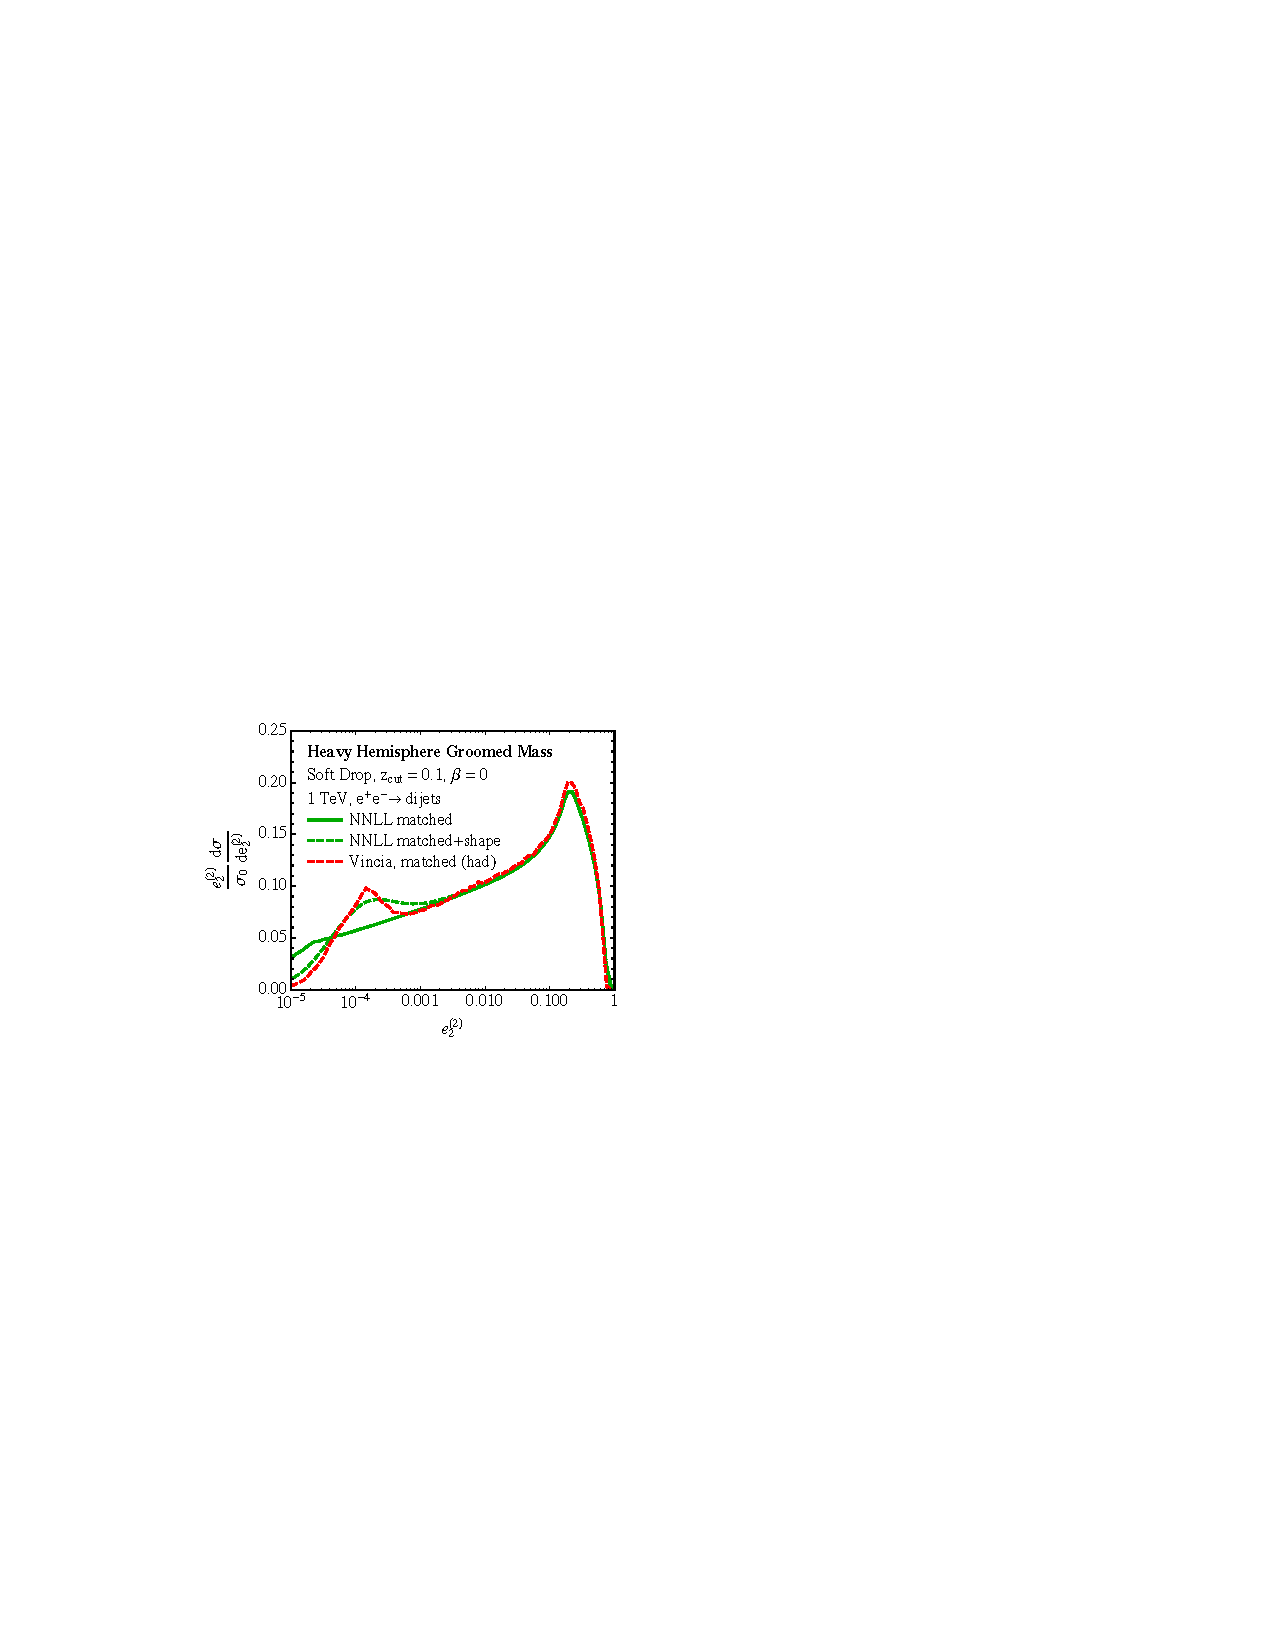
\includegraphics[width = 0.6\columnwidth]{figures/shape_function.pdf}
\end{center}
\caption{A plot showing the effects of non-perturbative corrections to the groomed jet mass. This illustrates first that the non-perturbative corrections are suppressed over a large range, and second that they take a very different form than for double logarithmic observables. Figure from \cite{Frye:2016aiz}. }
\label{fig:shape_function}
\end{figure}




Finally, while in this section we have so far focused on the effect of the grooming procedure on hadronization corrections, and a comparision to $e^+e^-$ event shapes, we must also emphasize that the grooming plays an important role in suppressing non-perturbative corrections from the underlying event. This is crucial for achieving a precision measurement in the $pp$ environment, since there is a limited theoretical understanding of the underlying event. Here we must rely purely on Monte Carlo model implementations of the underlying event.  Monte Carlo studies have shown that in the regime where one has perturbative control, underlying event is highly suppressed. This is again a significant benefit of groomed observables. 




%%%%%%%%%%%%%%%%%%%%%%%%%%%%%%%%%%%%%
\subsection{Perturbative Simplicity}
\label{sec:pertsimplicity}
%%%%%%%%%%%%%%%%%%%%%%%%%%%%%%%%%%%%%

By studying the analytic behavior of grooming on the jet mass, the authors of Ref.~\cite{Dasgupta:2013ihk} showed that grooming could be designed to enhance the simplicity and calculability of various jet shapes.  In particular, grooming significantly simplifies the perturbative resummation in the $pp$ environment in addition to suppressing NP corrections.  Calculations of the standard jet mass in $pp$ typically suffer from the following two perturbative difficulties
\begin{itemize}
\item Global color correlations, which complicate the structure of higher order soft functions.
\item Non-global logarithms \cite{Dasgupta:2001sh}, which complicate the perturbative structure for non-global measurements.
\end{itemize}
The jet mass was calculated in \cite{Jouttenus:2013hs} (\cite{arXiv:1207.1640}) for $H+$ jet with(out) a
veto on additional radiation, supplemented with arguments that
non-global effects are small. However, these two features highlight
that the ungroomed jet mass depends significantly on the particular
process that created the jet, significantly reducing its universality,
and complicating its structure in a busy $pp$ environment. We will see
that through the use of grooming we will be able to make the jet mass
nearly universal.


In \Ref{Frye:2016aiz} it was shown that for $\ecf{2}{\alpha} \ll \zcut \ll 1$,  we can express the cross section for the groomed angularity as
\begin{align}\label{eq:fac_pp_e2}
\frac{d\sigma^{pp}}{d\ecf{2}{\alpha}}=\sum\limits_{k=q,\bar q, g}D_k(p_T^{\text{min}}, y_\text{max}, \zcut, R) S_{C,k}(\zcut, \ecf{2}{\alpha})\otimes J_k (\ecf{2}{\alpha})\,,
\end{align}
\noindent where $S_{C,k}$ is the soft function and $J_k$ is the jet function.  The function $D_k$ depends on the parton flavor, and can be interpreted as the quark and gluon fractions. While the quark and gluon fractions are generally not IRC safe quantities, in this limit they are well defined, 
\begin{align}
f_J=\sum\limits_{i\in J_{\text{SD}}} f_i\,,
\end{align}
with $f_q=1$, $f_{\bar q}=-1$, $f_g=0$, and $J_{\text{SD}}$ are the constituents of the groomed jet. The grooming procedure makes this IRC safe. These fractions are independent of the value of the jet mass observable. These coefficients can be extracted from fixed order Monte Carlo programs, for example MCFM \cite{Campbell:1999ah,Campbell:2010ff,Campbell:2011bn}.



This formula has a number of remarkable consequences. In the resummation region, we see that there are no non-global logarithms, and there are no global color correlations. The collinear soft and jet functions depend only on the jet flavor. They are therefore identical to in the case of groomed jets in $e^+e^-$. In the resummation region, the grooming algorithm has therefore allowed the jet to be isolated from its $pp$ environment, and all that is required are the quark and gluon fractions. 


It is important to emphasize that this simplification does not occur
throughout the entire distribution. In particular, for $m \gg Q\zcut$,
it does not hold. However, this is the fixed order region, where we
can match to standard fixed order perturbation theory. This matching
has been performed to (N)NLO for dijets ($V$+jets)
\cite{Frye:2016aiz,Marzani:2017kqd,Marzani:2017mva}.  Ideally this would be done using $2\to 3$ matrix
elements at NNLO, which are just now becoming available
\cite{Gehrmann:2015bfy,Dunbar:2016aux,Badger:2013yda,Badger:2017jhb,Abreu:2017hqn}.



%\info{IAN}
%
%\begin{itemize}
%\item grooming original purpose: reduce sensitivity to soft-wide angle radiation
%\item it obviously reduces the impact of UE and pile-up in pp collision
%\item what about hadronization? at first sight less obvious because we get rid of soft radiation but we also reduce the effective radius. Competing effects?
%\item however it helps with hadronization too: parametric understanding (here there is some calculation in mMDT paper and Harvard paper too). Some unpublished studies exist on  for $\beta>0$ by Gregory, Lais and SM. 
%\item Abundant MC evidence that helps
%\item Open question: any deeper understanding in terms of shape functions?
%\end{itemize}

%Comparison to shape function in thrust.  Grooming gives different sensitivity to NP effects.
%
%In standard thrust fits, whole distribution shifts from NP.  Degenerate with $\alpha_s$ shift, hard to disentangle.
%
%Grooming pushes NP effects to separate region.  Separation of NP region, resummation region, fixed order regime (at high enough jet $p_T$).


%%%%%%%%%%%%%%%%%%%%%%%%%%%%%%%%%%%%%%
%\subsection{Process Independence at Hadron Colliders ($pp$)}
%%%%%%%%%%%%%%%%%%%%%%%%%%%%%%%%%%%%%%
%
%\info{IAN}
%
%clearly there still is some process-dependence, in terms of q/g fractions as well as hard coefficients. It is however much reduced.
%compare to issue of PDF, 3-jet over 2-jet, ECF extractions
%Grooming removes soft correlations: it ``turns the LHC into an e$^+$e$^-$ machine (too strong?)
%Related:  Grooming remove NGLs and other contamination. It makes things easier to calculate. 
%


%%%%%%%%%%%%%%%%%%%%%%%%%%%%%%%%%%%%%
\subsection{Pileup Resilience}
%%%%%%%%%%%%%%%%%%%%%%%%%%%%%%%%%%%%%

Arguably the biggest experimental challenge for precision physics at a high luminosity $pp$ collider is noise from \textit{pileup}: multiple nearly simultaneous proton-proton collisions.  Jet shapes are particularly sensitive to pileup; for example, the jet mass scales as $\mathcal{O}(R^4)$~\cite{Salam:2009jx} for the jet area $A$~\cite{Cacciari:2008gn} (whereas the jet $p_\text{T}$ scales linearly with $A$).  The jet-areas subtraction that works well for $p_\text{T}$ has been extended to event shapes~\cite{Soyez:2012hv}, but must be re-calibrated per observable.  Constituent-based pileup subtraction schemes~\cite{Cacciari:2014gra,Krohn:2013lba,Bertolini:2014bba,Berta:2014eza,Komiske:2017ubm} show great promise and are actively being studied and adapted to the actual experimental settings~\cite{CMS-PAS-JME-14-001,CMS-DP-2015-034,ATLAS-CONF-2017-065,ATL-PHYS-PUB-2017-020,Aad:2015ina}.  However, even without constituent-based subtraction techniques, there is a large reduction in pileup sensitivity to jet substructure from grooming~\cite{CMS-PAS-JME-14-001,Aad:2015rpa,Aad:2015ina,Altheimer:2013yza}.  Grooming systematically removes soft and wide-angle radiation, which is exactly the profile characteristic of pileup.   Even with extreme levels of pileup (up to 300 collisions), grooming can preserve the distribution of the jet mass distribution~\cite{JetSubstructureECFA2014}.   Despite the power of grooming for pileup suppression, there is still a residual degradation of resolution with increased levels of pileup which makes precision jet substructure measurements challenging at high instantaneous luminosity.  Track-based observables are robust to pileup because their vertex of origin can be well-distinguished from pileup vertices.  Precision track-based substructure observables have been calculated~\cite{Krohn:2012fg,Waalewijn:2012sv,Chang:2013rca,Elder:2017bkd}, but typically require universal non-perturbative input.  It may be interesting to do a track- and jet substructure-based extraction of $\alpha_s$, but this is left as a possibility for future work.
